\subsection{Smooth solutions}

Tests over a sequence of uniform meshes have been conducted to verify the algorithm's performance, confirming that:

\begin{gather} \label{trends}
    \lVert u - u^k_h \rVert_{\LT(\Omega)} \approx h^{k + 1}, \\
    \lVert u - u^k_h \rVert_{DG} \approx h^k.
\end{gather}

These results were obtained by selecting a smooth function as exact solution such as the following:

\begin{gather}
    u(x, y) = \sin(2 \pi x) \cos(2 \pi y),
\end{gather}

which leads to:

\begin{gather}
    f(x, y) = -\Delta u(x, y) = 8 \pi^2 \sin(2 \pi x) \cos(2 \pi y),
\end{gather}

and non-homogeneous Dirichlet boundary conditions given by the exact solution itself.

\newpage
\subsubsection{Errors}

The following shows the error trends for the $\LT$ and $DG$ errors over sequences of uniform meshes over the square and L-shaped domains. The relations presented in \eqref{trends} have been confirmed.

\begin{figure}[!ht]
	\centering
	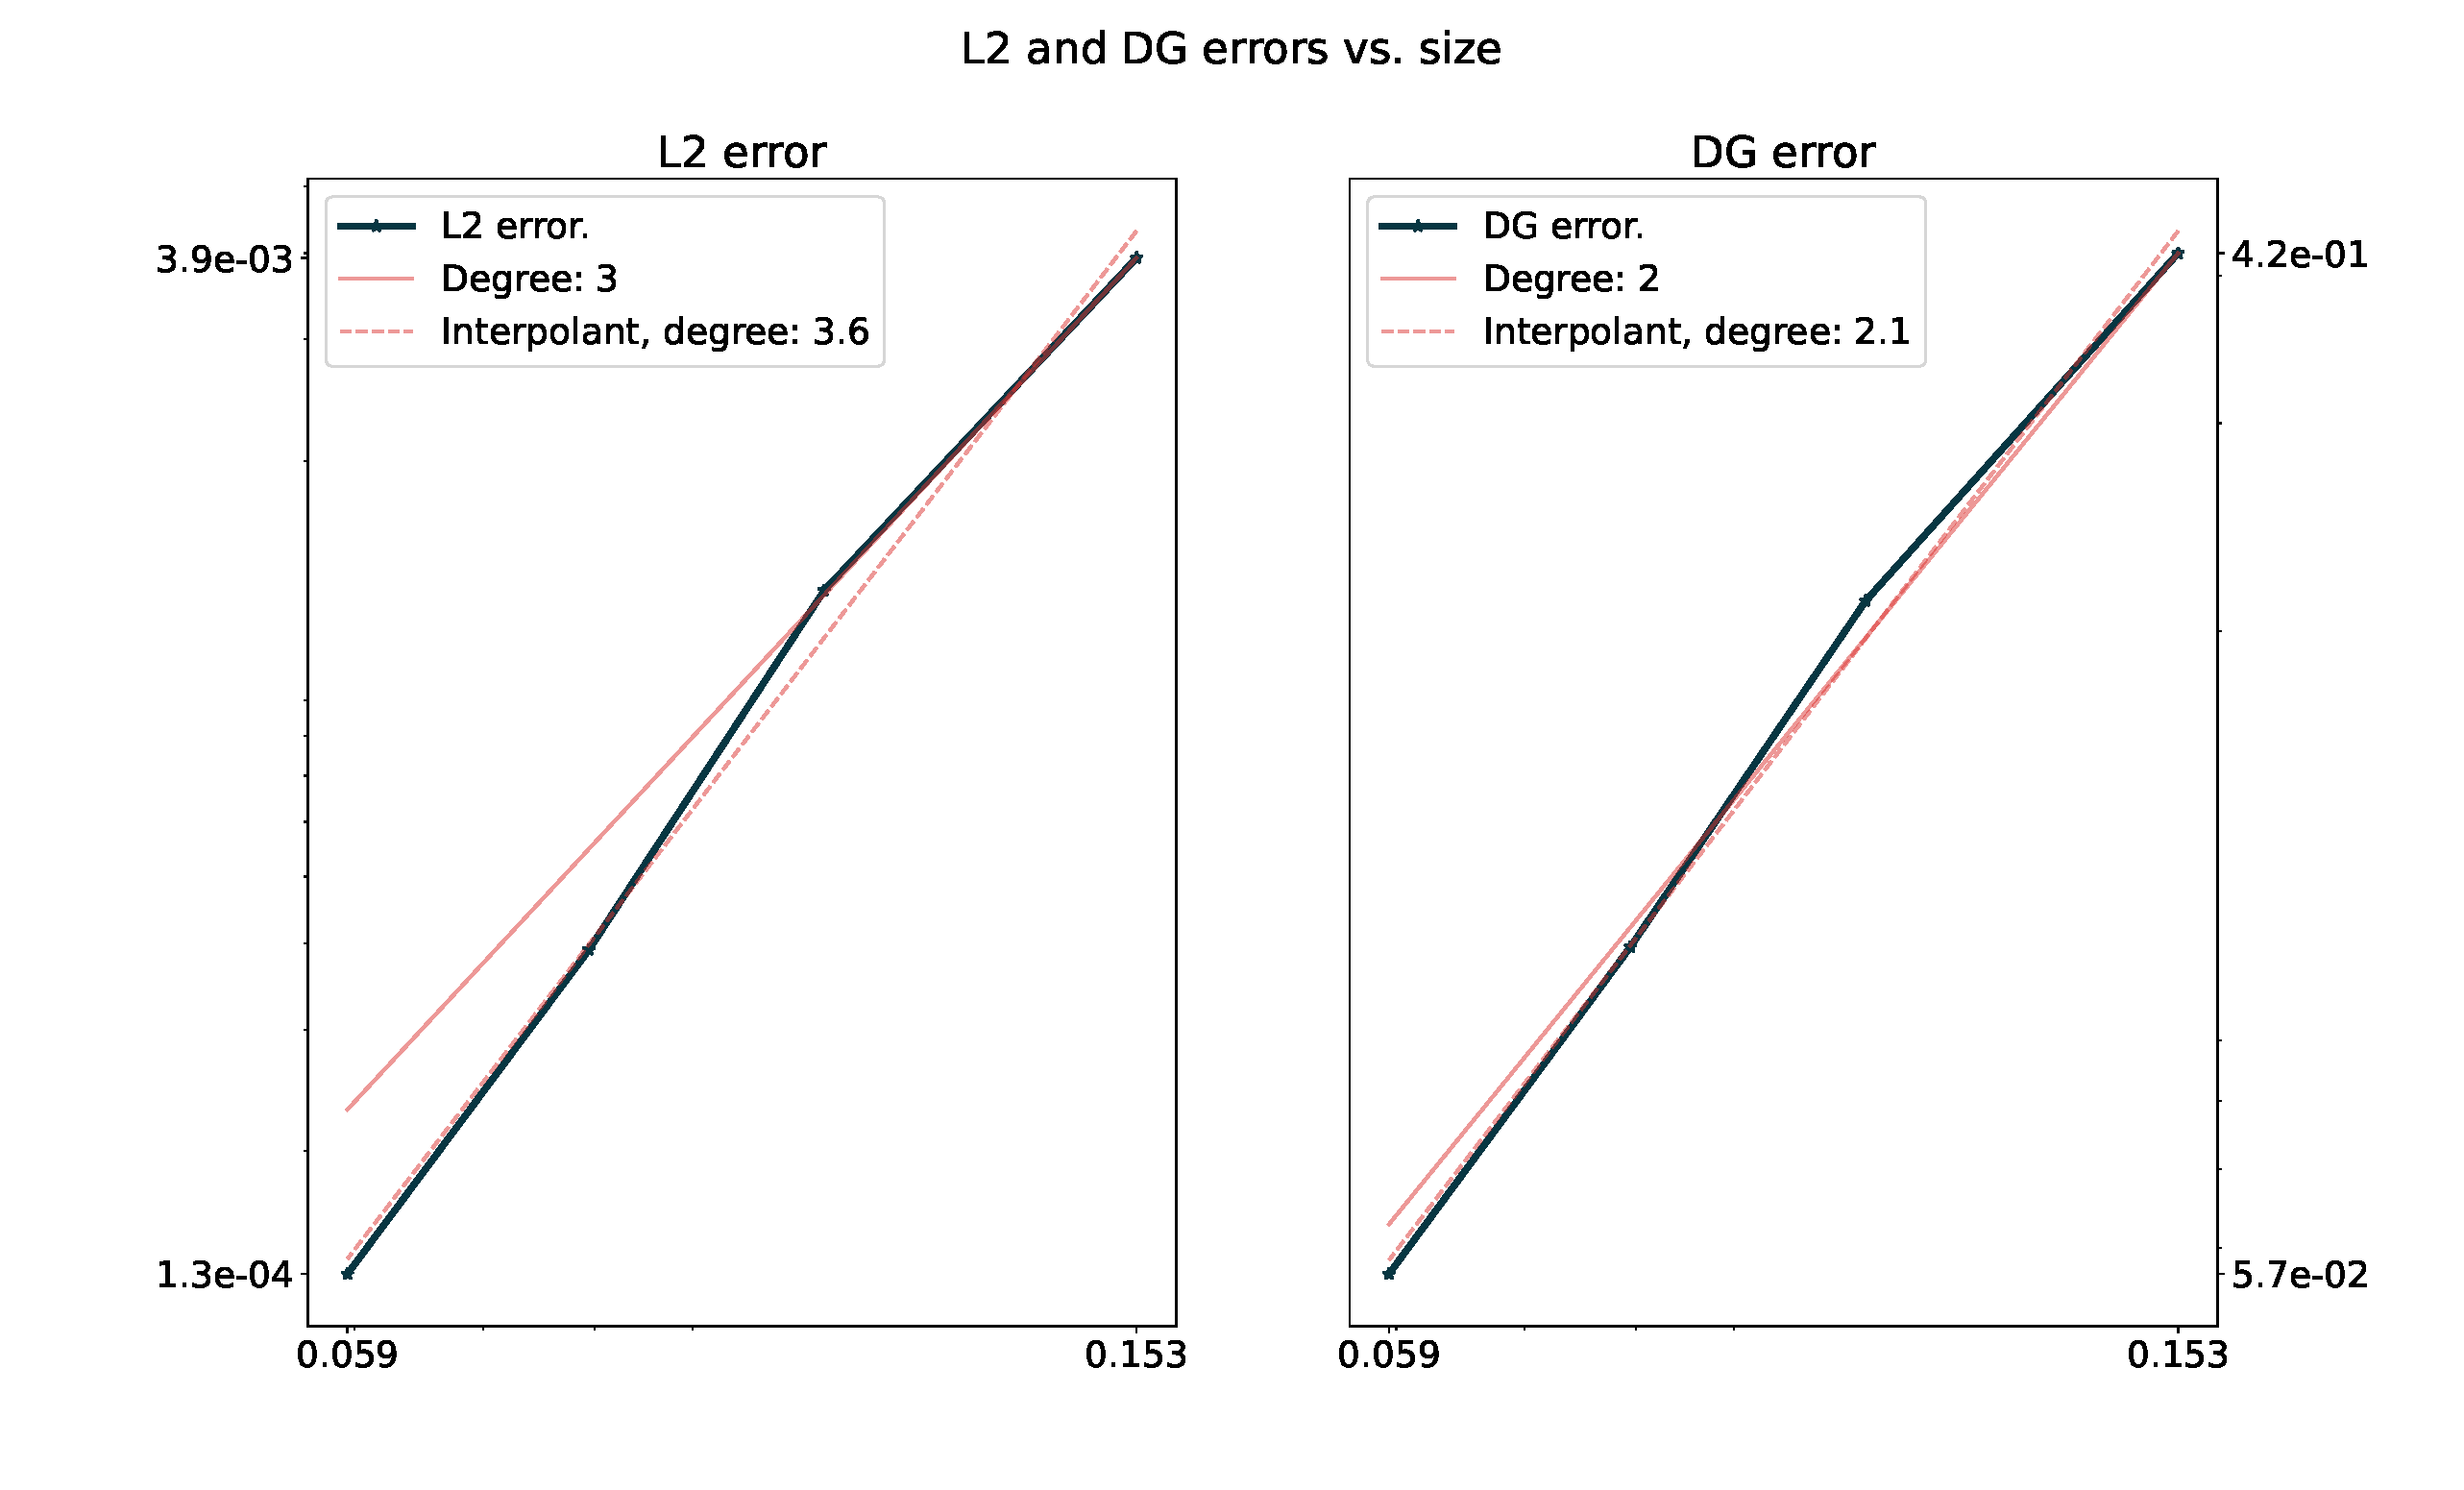
\includegraphics[trim=0cm 0.5cm 0cm 2cm, clip, width=16cm]{square_uniform.pdf}
    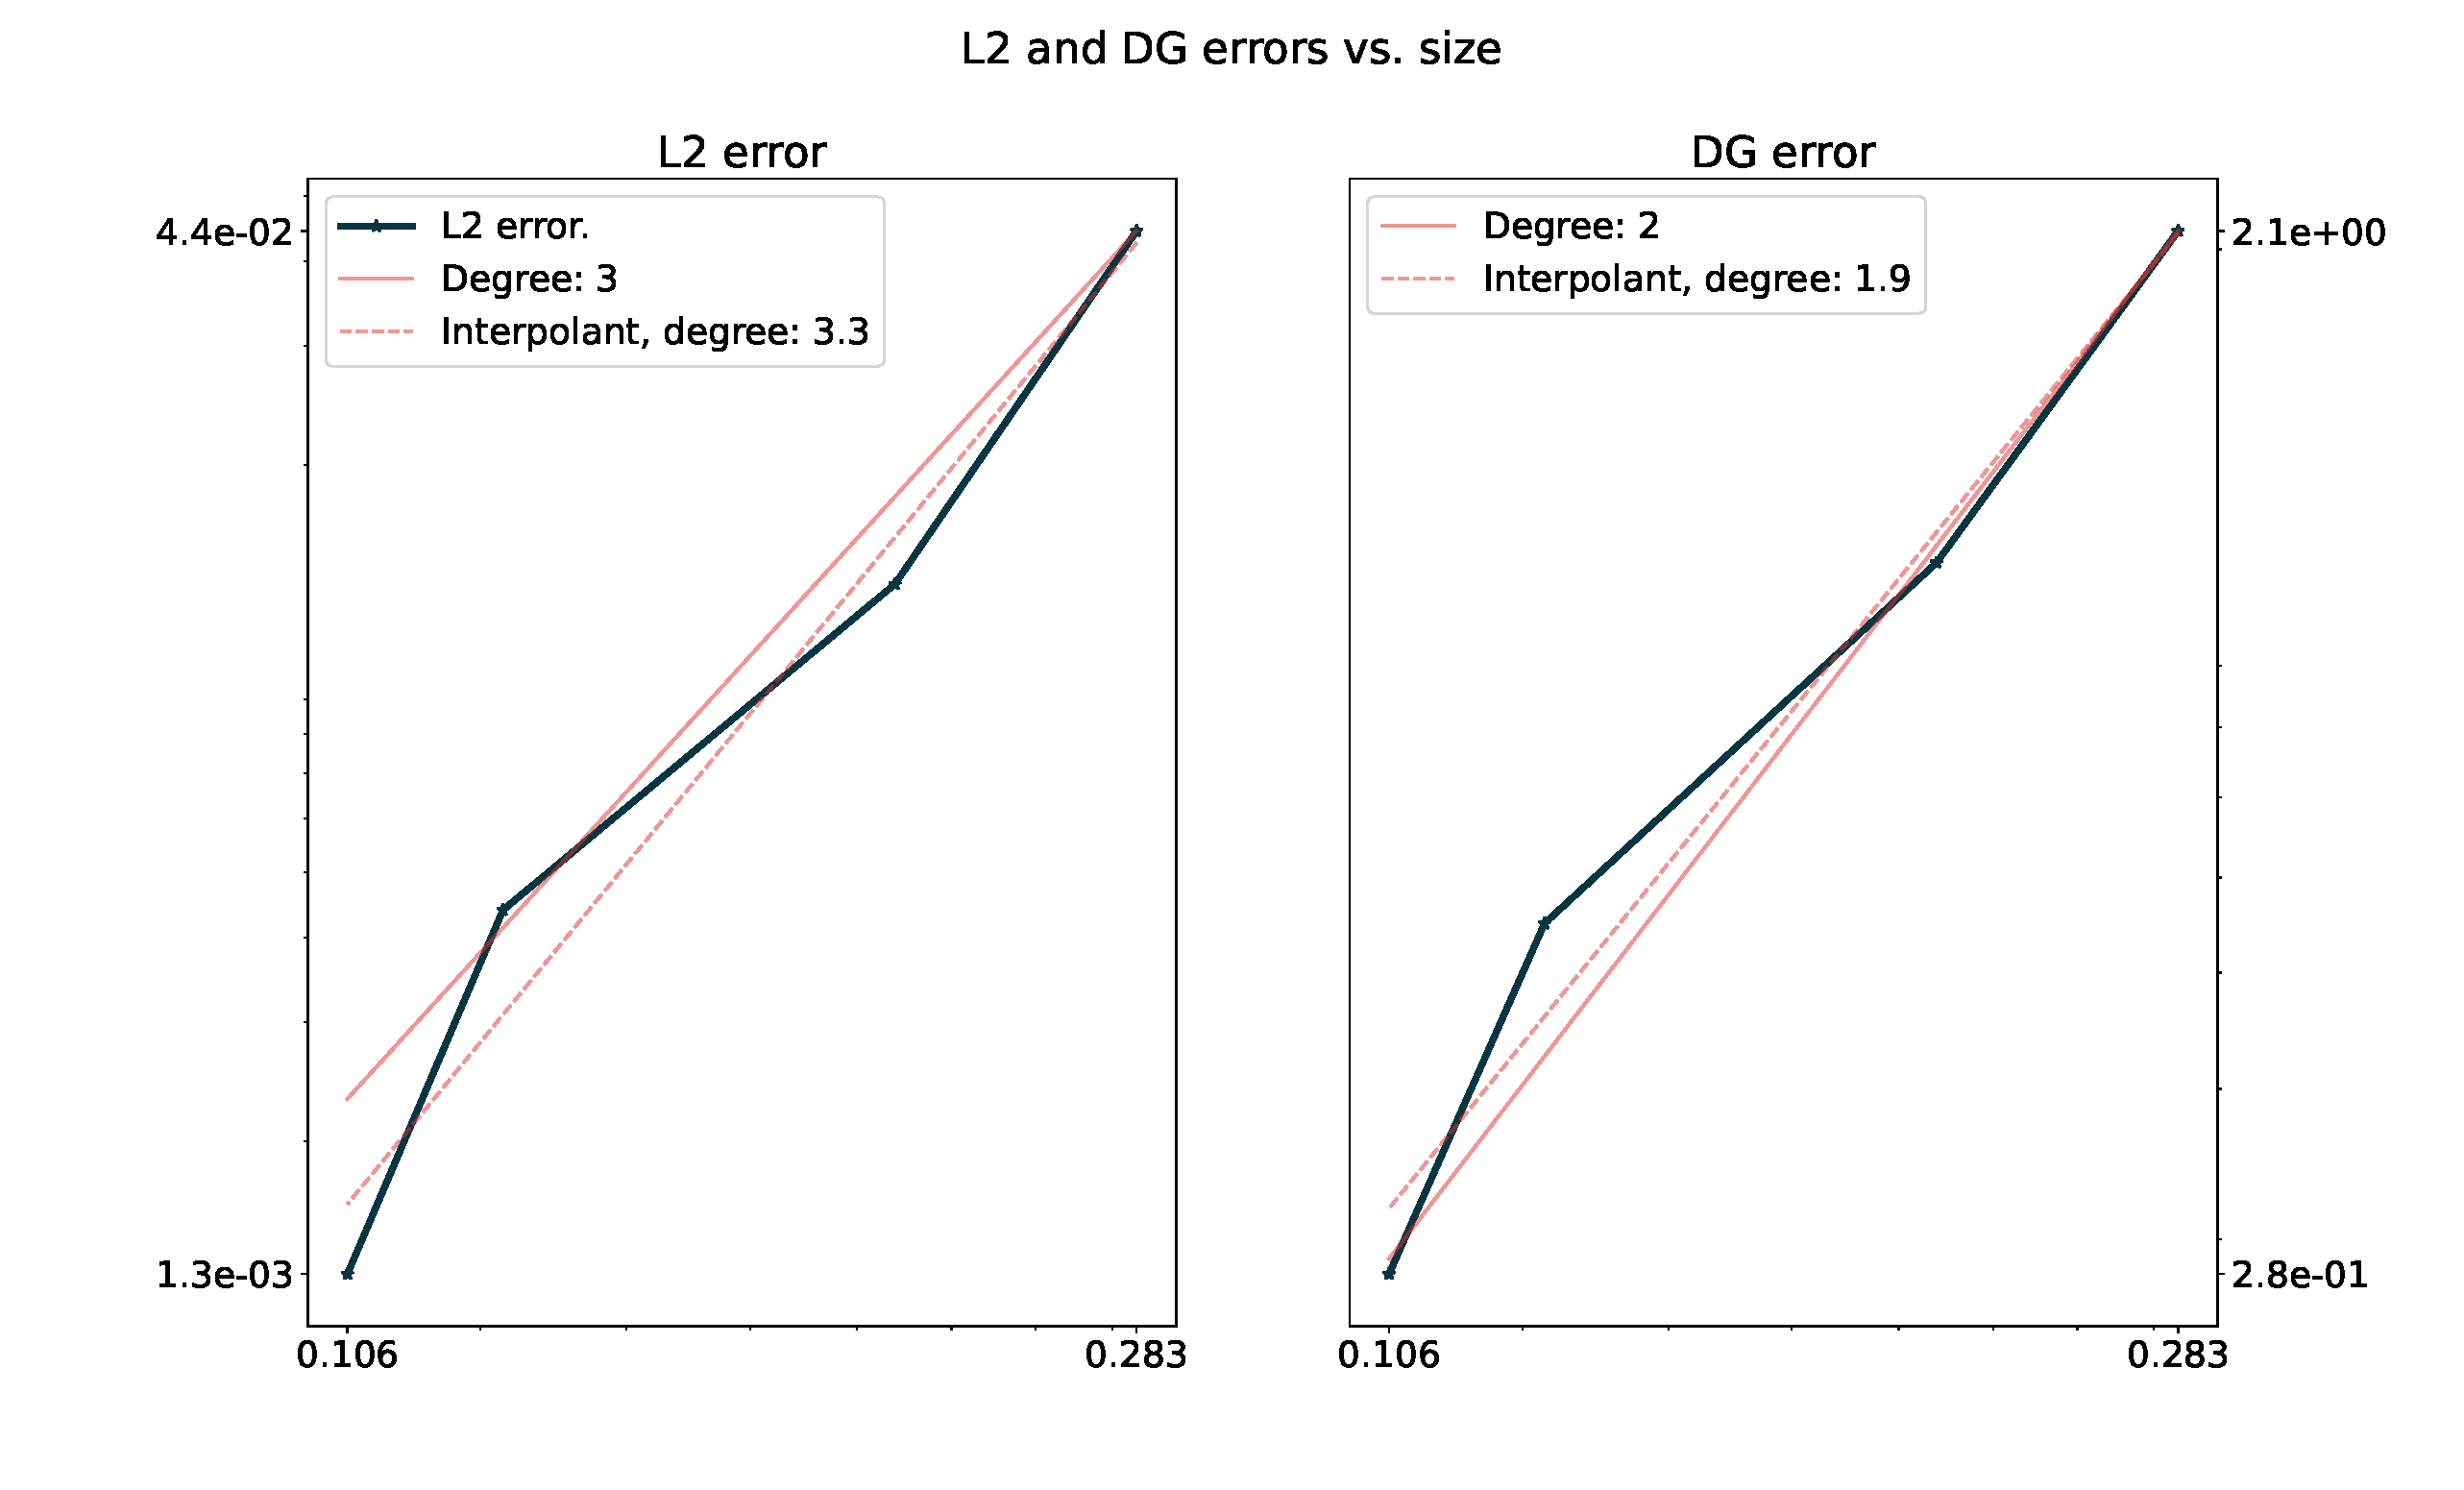
\includegraphics[trim=0cm 0.5cm 0cm 2cm, clip, width=16cm]{lshape_uniform.pdf}
	\caption{$\LT$ and DG errors versus mesh size on a sequence of uniform meshes over a square domain (top) and an L-shaped domain (bottom), $k = 2$ and $N \in \{100, 200, 400, 800\}$.}
\end{figure}

\newpage
\subsubsection{Solutions}

The following shows a scatter plot of the numerical solution $u^k_h$, the exact solution $u$, and the error $|u - u^k_h|$ over the quadrature nodes.

\begin{figure}[!ht]
	\centering
	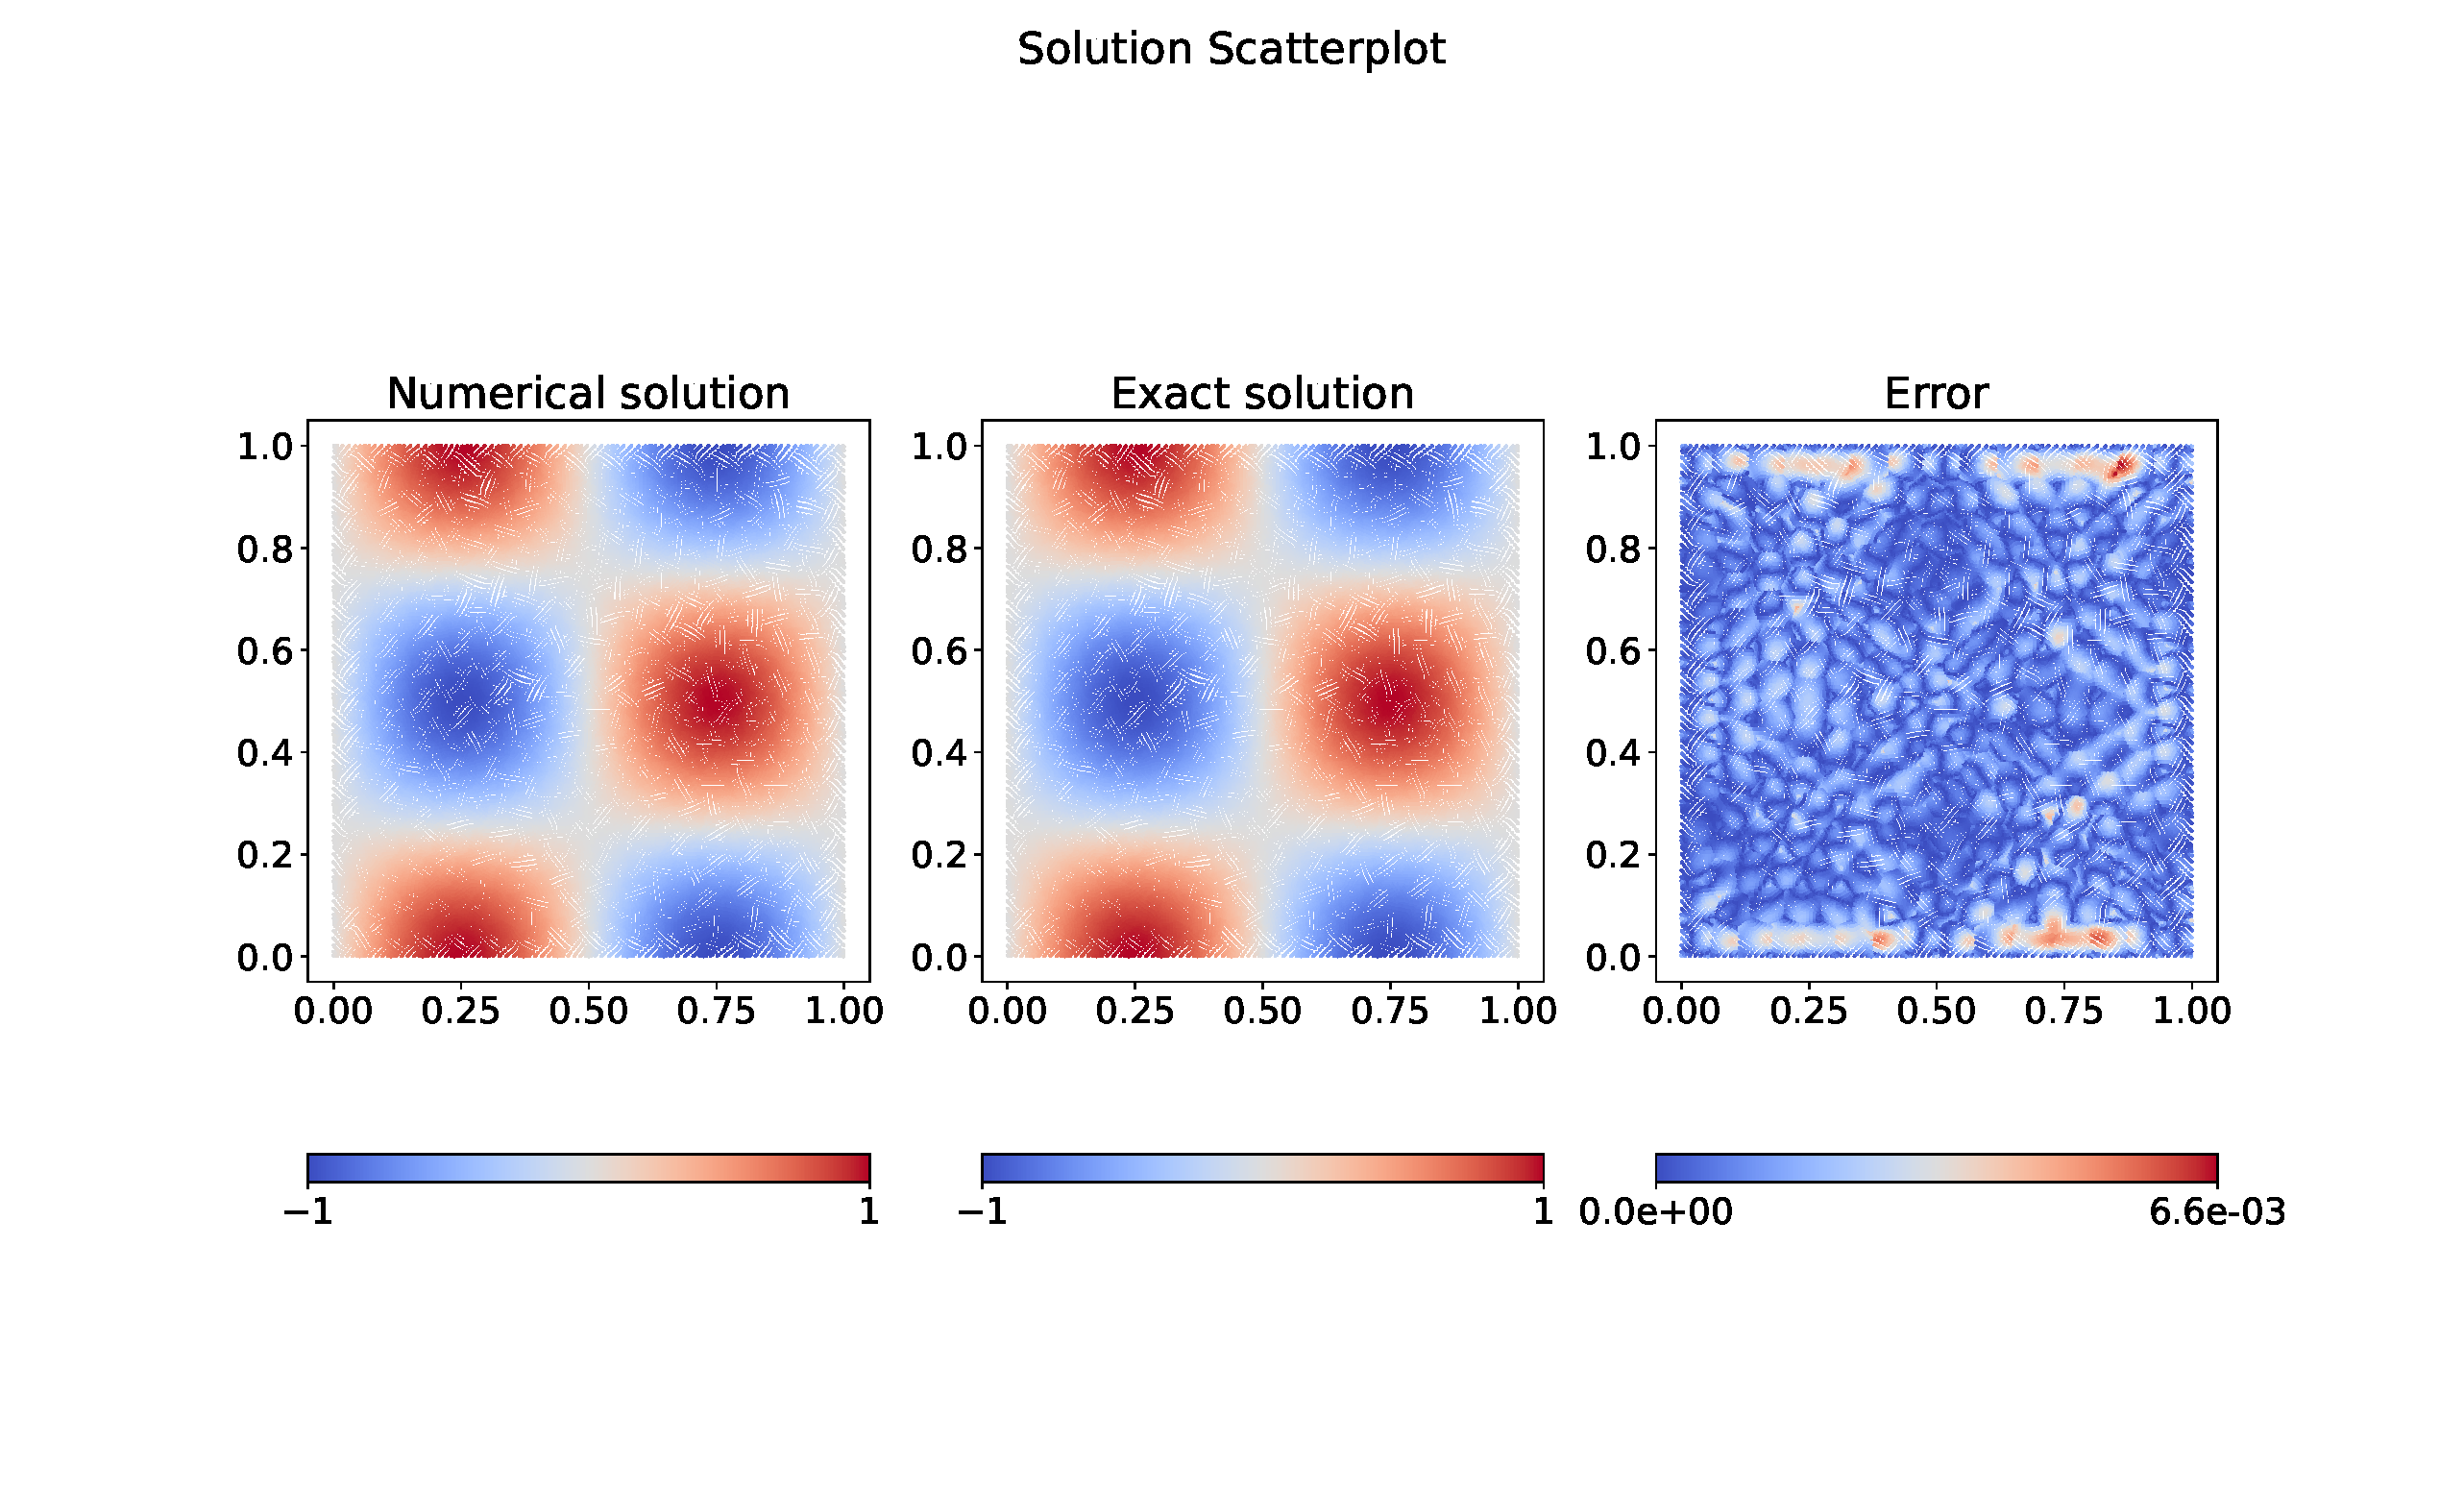
\includegraphics[trim=0cm 2.5cm 0cm 5cm, clip, width=16cm]{square_200_sol.pdf}
    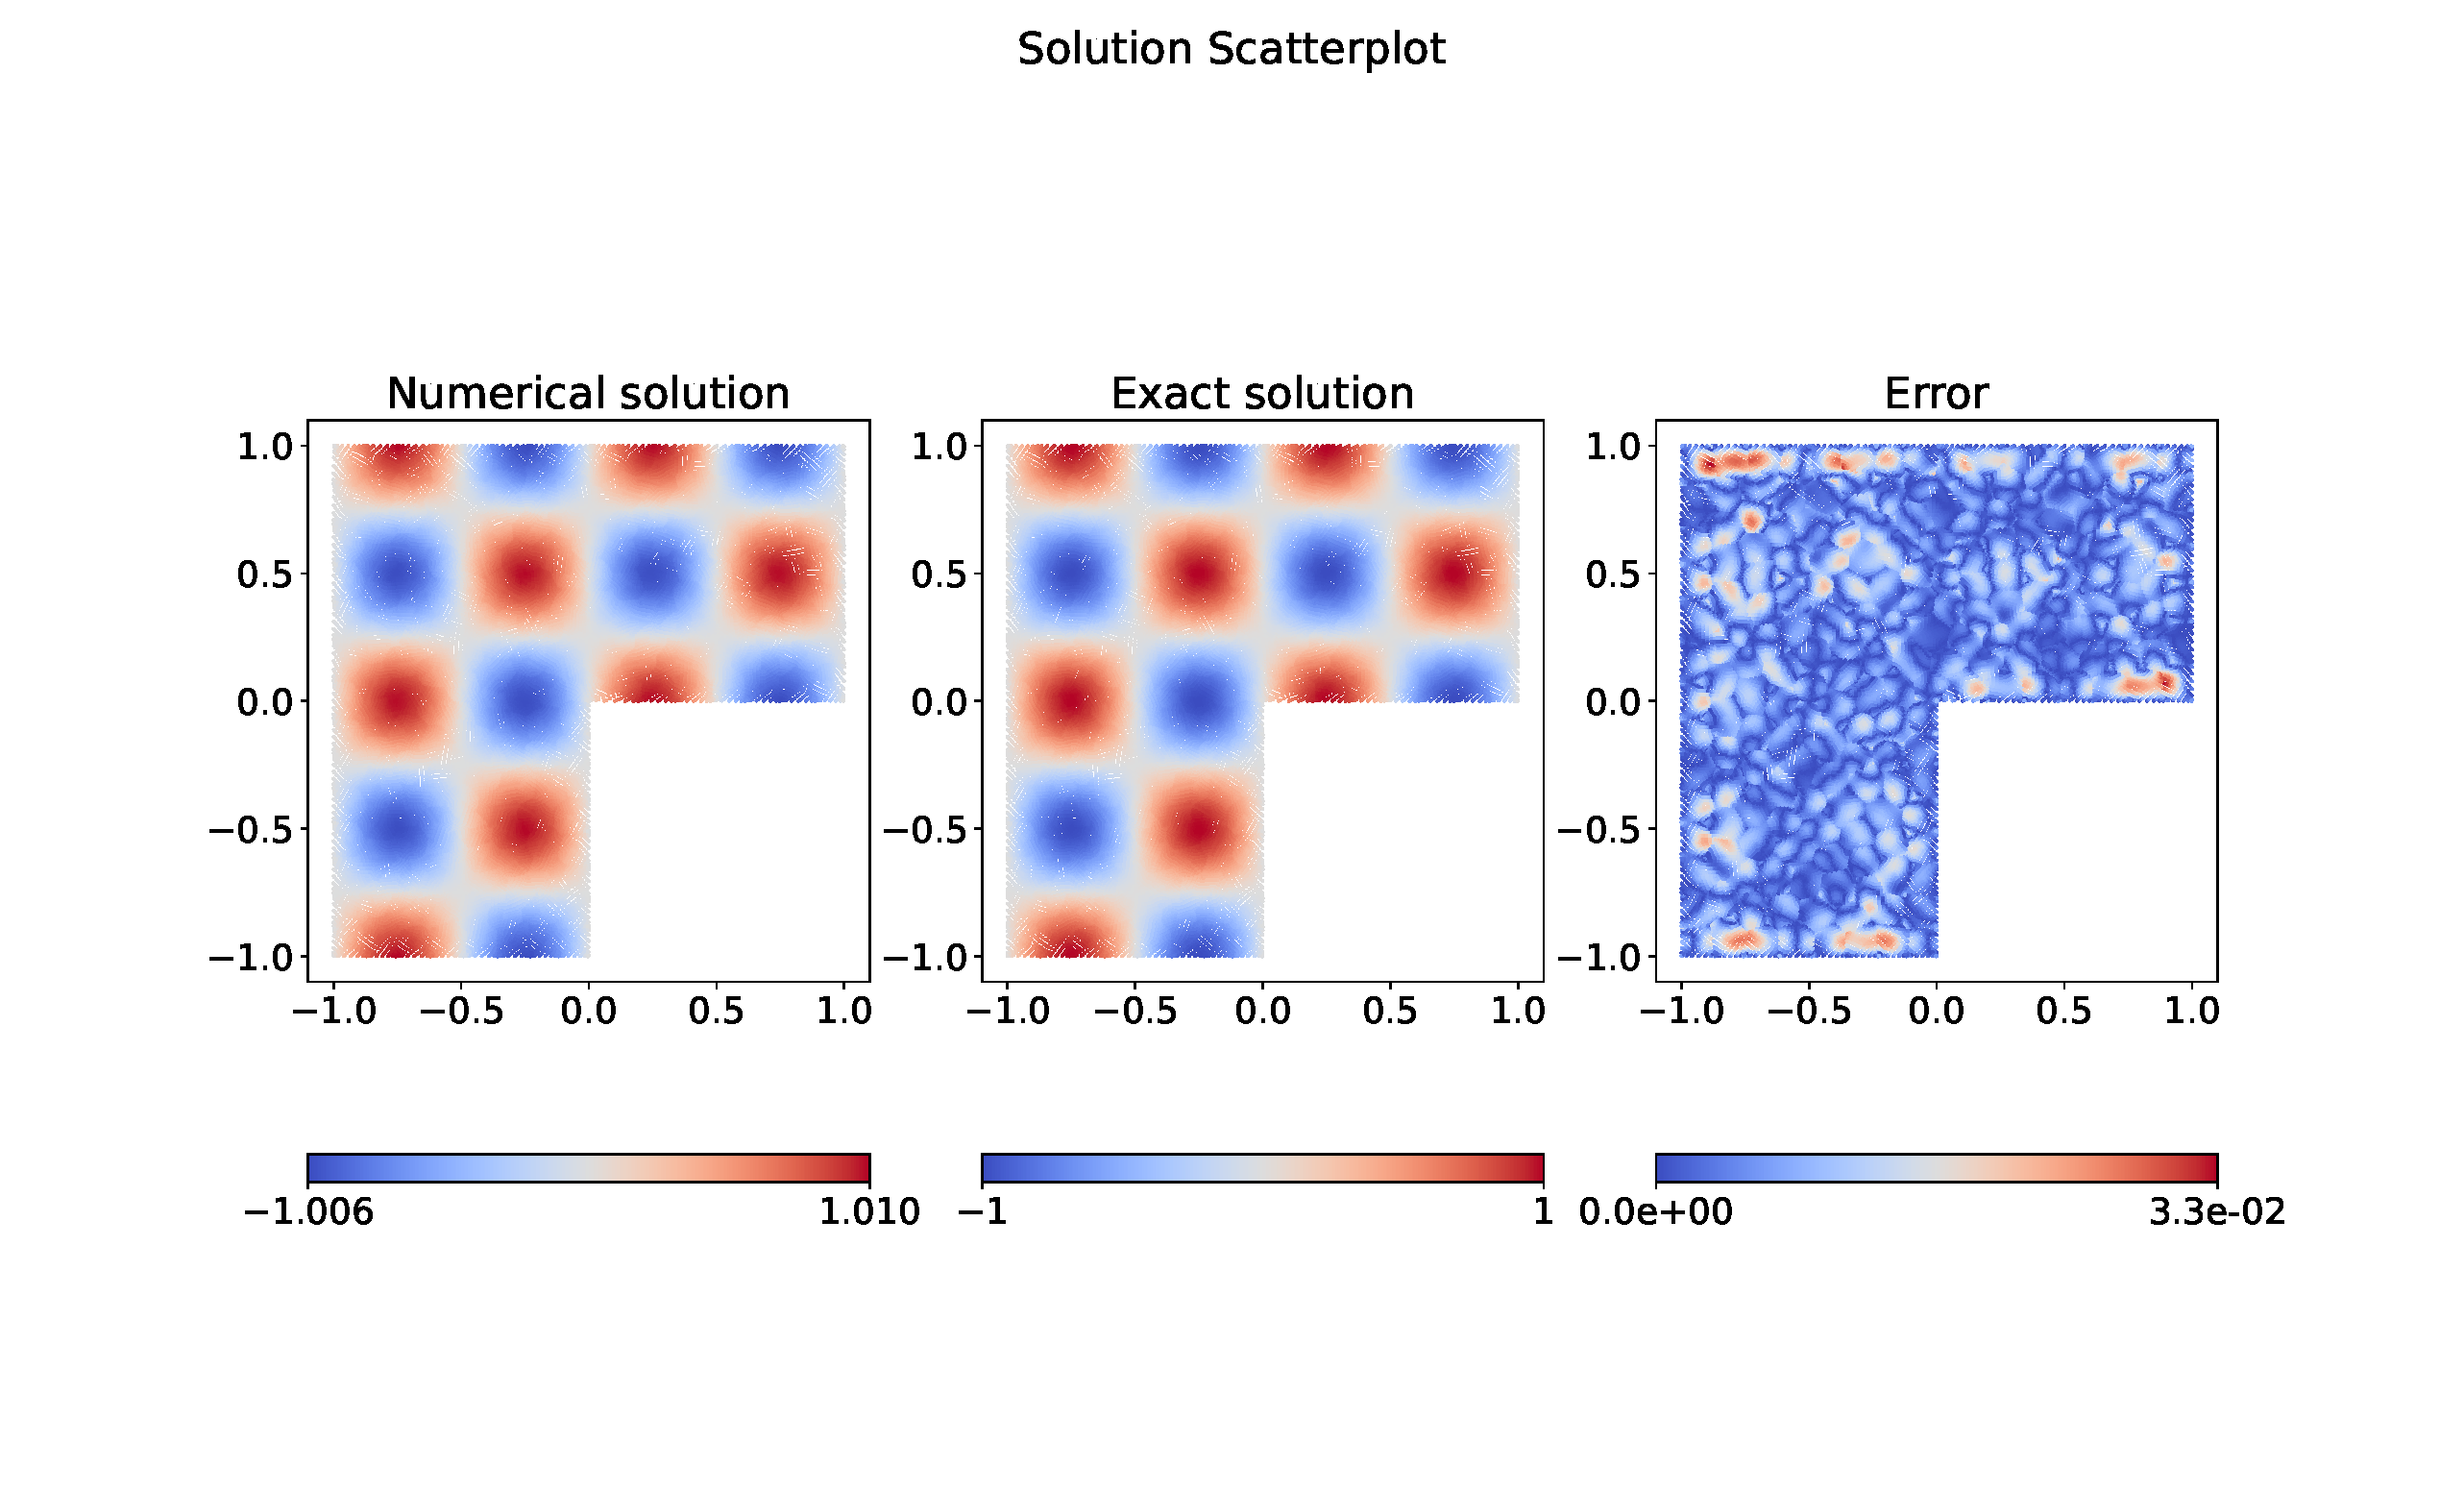
\includegraphics[trim=0cm 2.5cm 0cm 5cm, clip, width=16cm]{lshape_200_sol.pdf}
	\caption{Solution plot over a square domain (top) and an L-shaped domain (bottom), $N = 200$ and $k = 2$.}
\end{figure}

\newpage
\subsection{Pathological solutions}

Tests over a sequence of uniform meshes, using pathological functions as exact solutions, highlight the need for an adaptive algorithm.

\cite{Antonietti2013} The pathological function for the square domain is:

\begin{gather}
    u(x, y) = \frac{1 - e^{-100x}}{1 - e^{-100}} \sin(\pi y) (1 - x),
\end{gather}

which exhibits a strong boundary layer along the line $x = 0$.

For the L-shaped domain, the pathological function is:

\begin{gather}
    u(\rho, \theta) = \rho^{2 / 3} \sin\left(\frac{2 \theta}{3}\right),
\end{gather}

for which we have $f = 0$ and we know that $u$ is analytical in $\Omega \setminus \Vector{0}$, but $\grad{u}$ is singular at the origin.

\newpage
\subsubsection{Errors}

\begin{figure}[!ht]
	\centering
	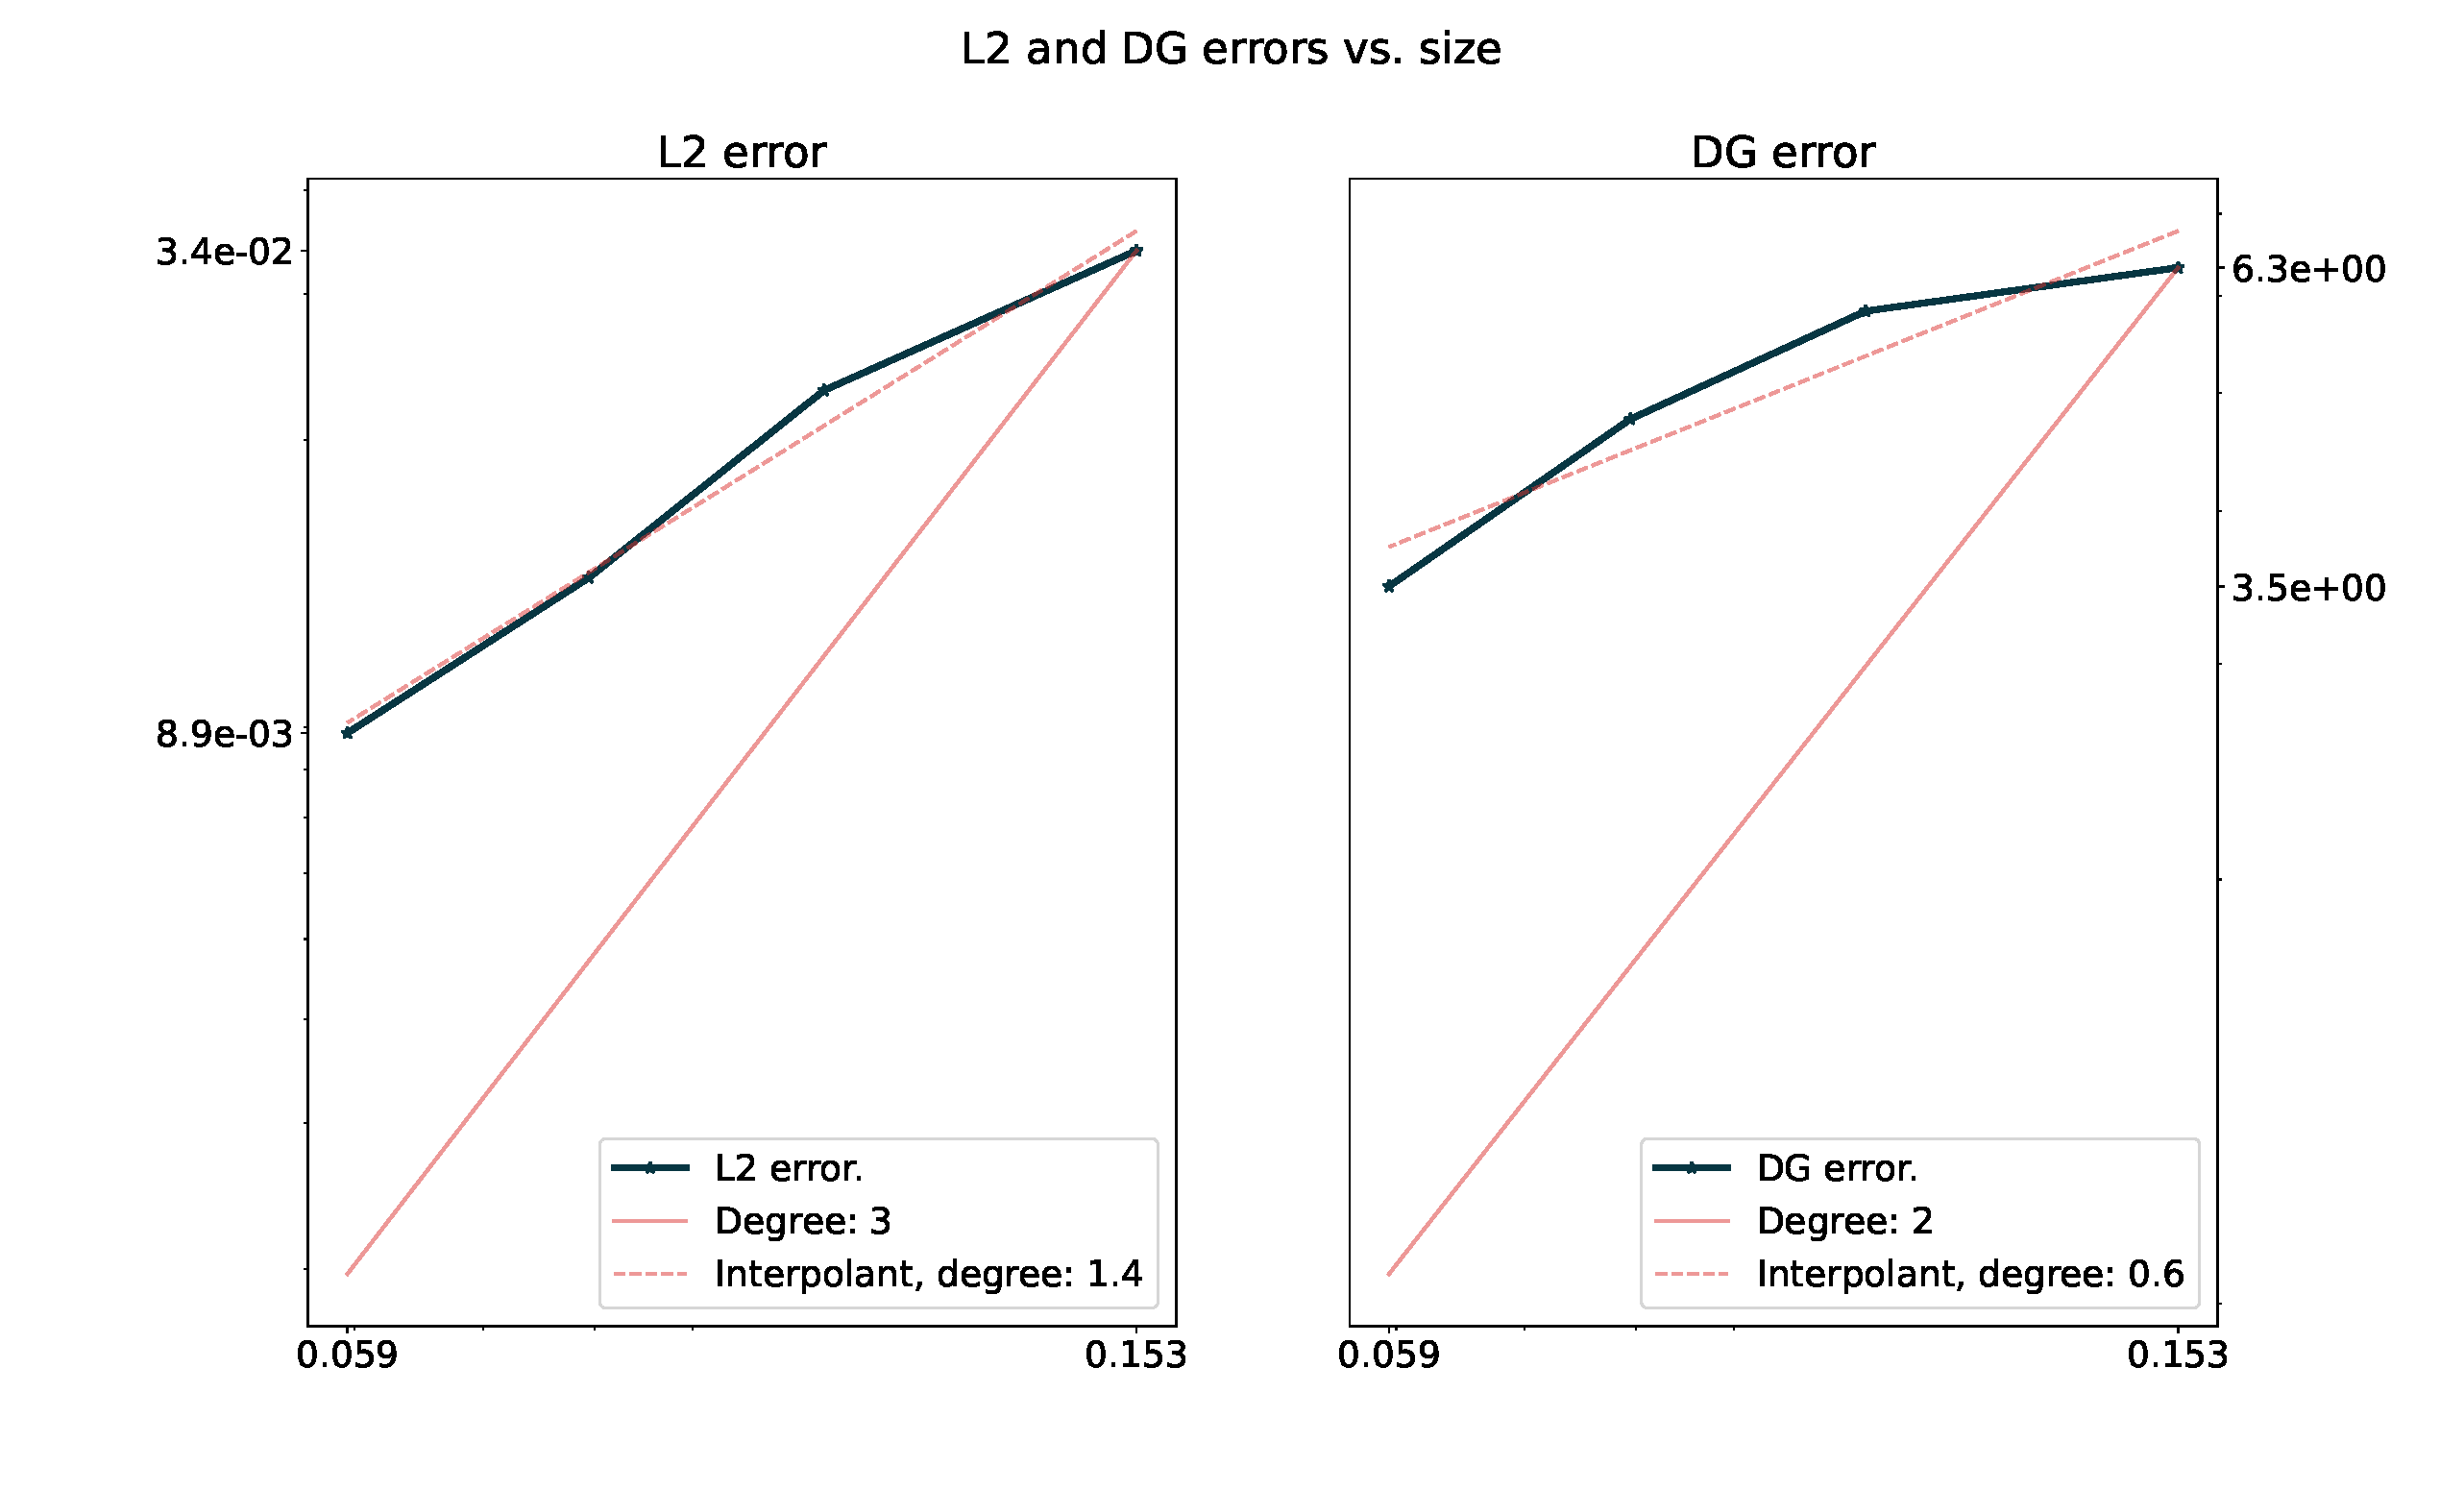
\includegraphics[trim=0cm 0.5cm 0cm 2cm, clip, width=16cm]{square_uniform_pat.pdf}
    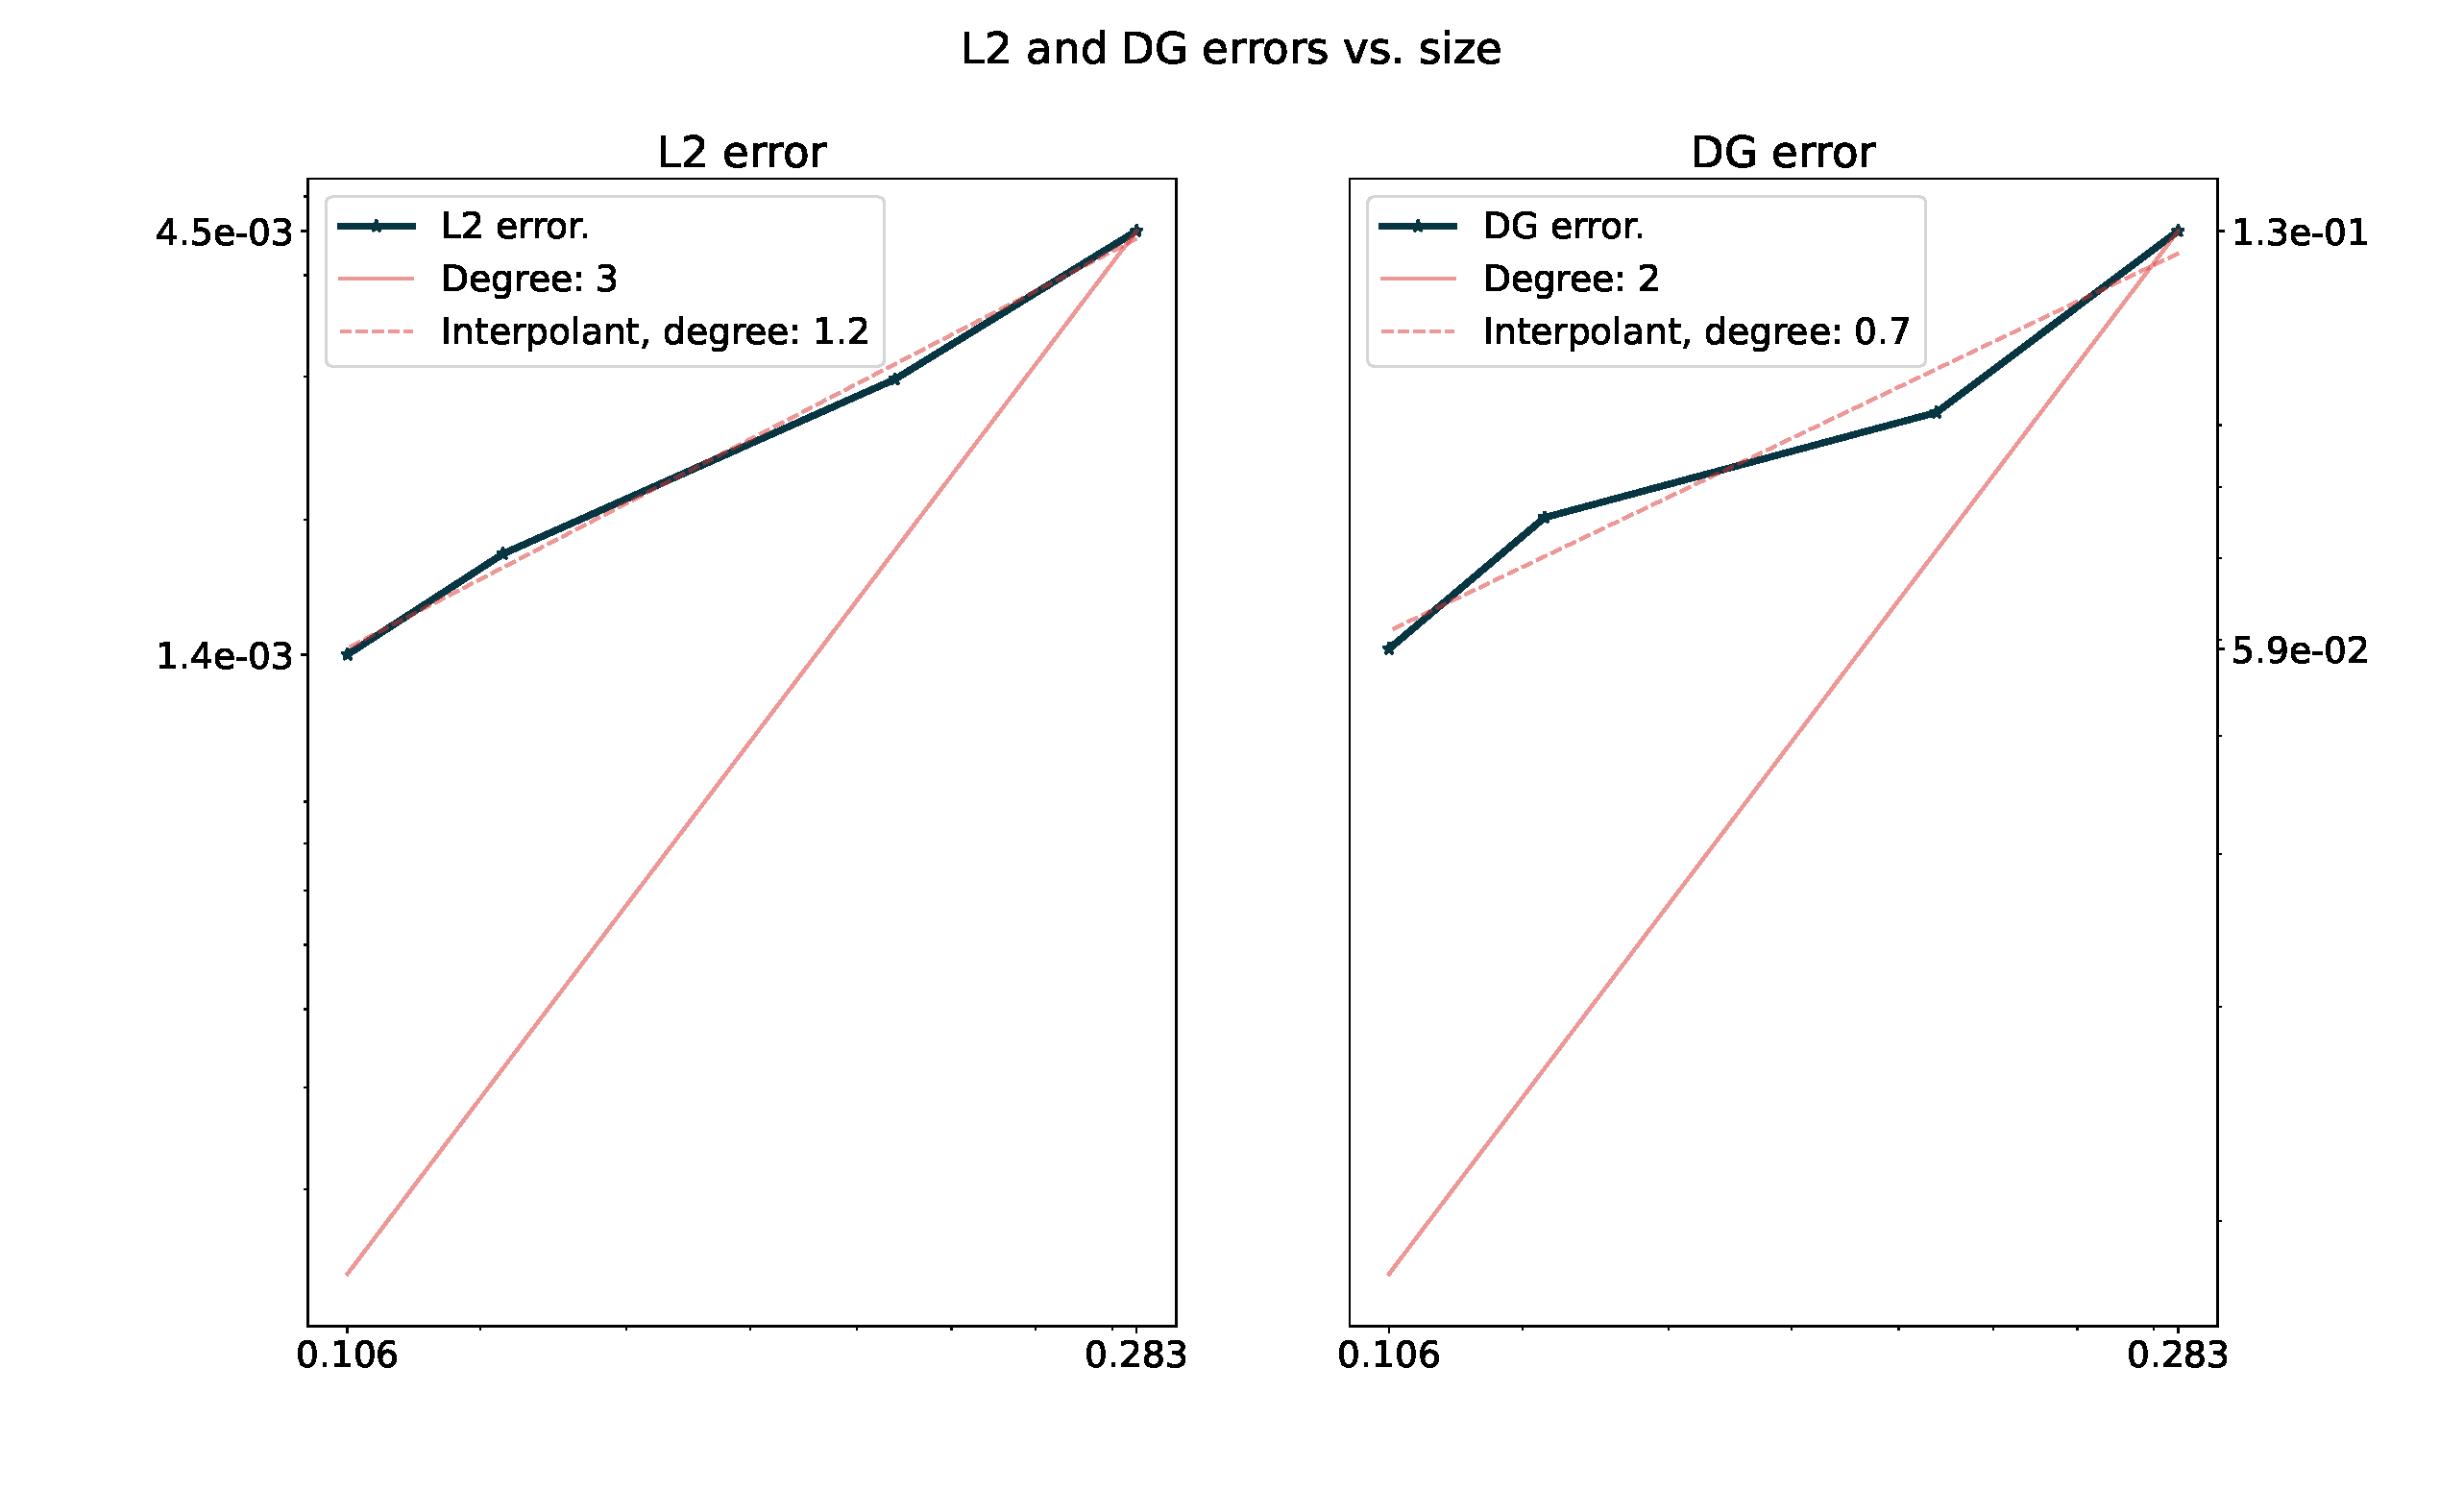
\includegraphics[trim=0cm 0.5cm 0cm 2cm, clip, width=16cm]{lshape_uniform_pat.pdf}
	\caption{$\LT$ and DG errors versus mesh size on a sequence of uniform meshes over a square domain (top) and an L-shaped domain (bottom), $k = 2$ and $N \in \{100, 200, 400, 800\}$.}
\end{figure}

\newpage
\subsubsection{Solutions}

The following plot shows that the error in these particular solutions is strongly localized, indicating that uniform refinement cannot perform optimally, also considering its rapidly growing computational cost.

\begin{figure}[!ht]
	\centering
	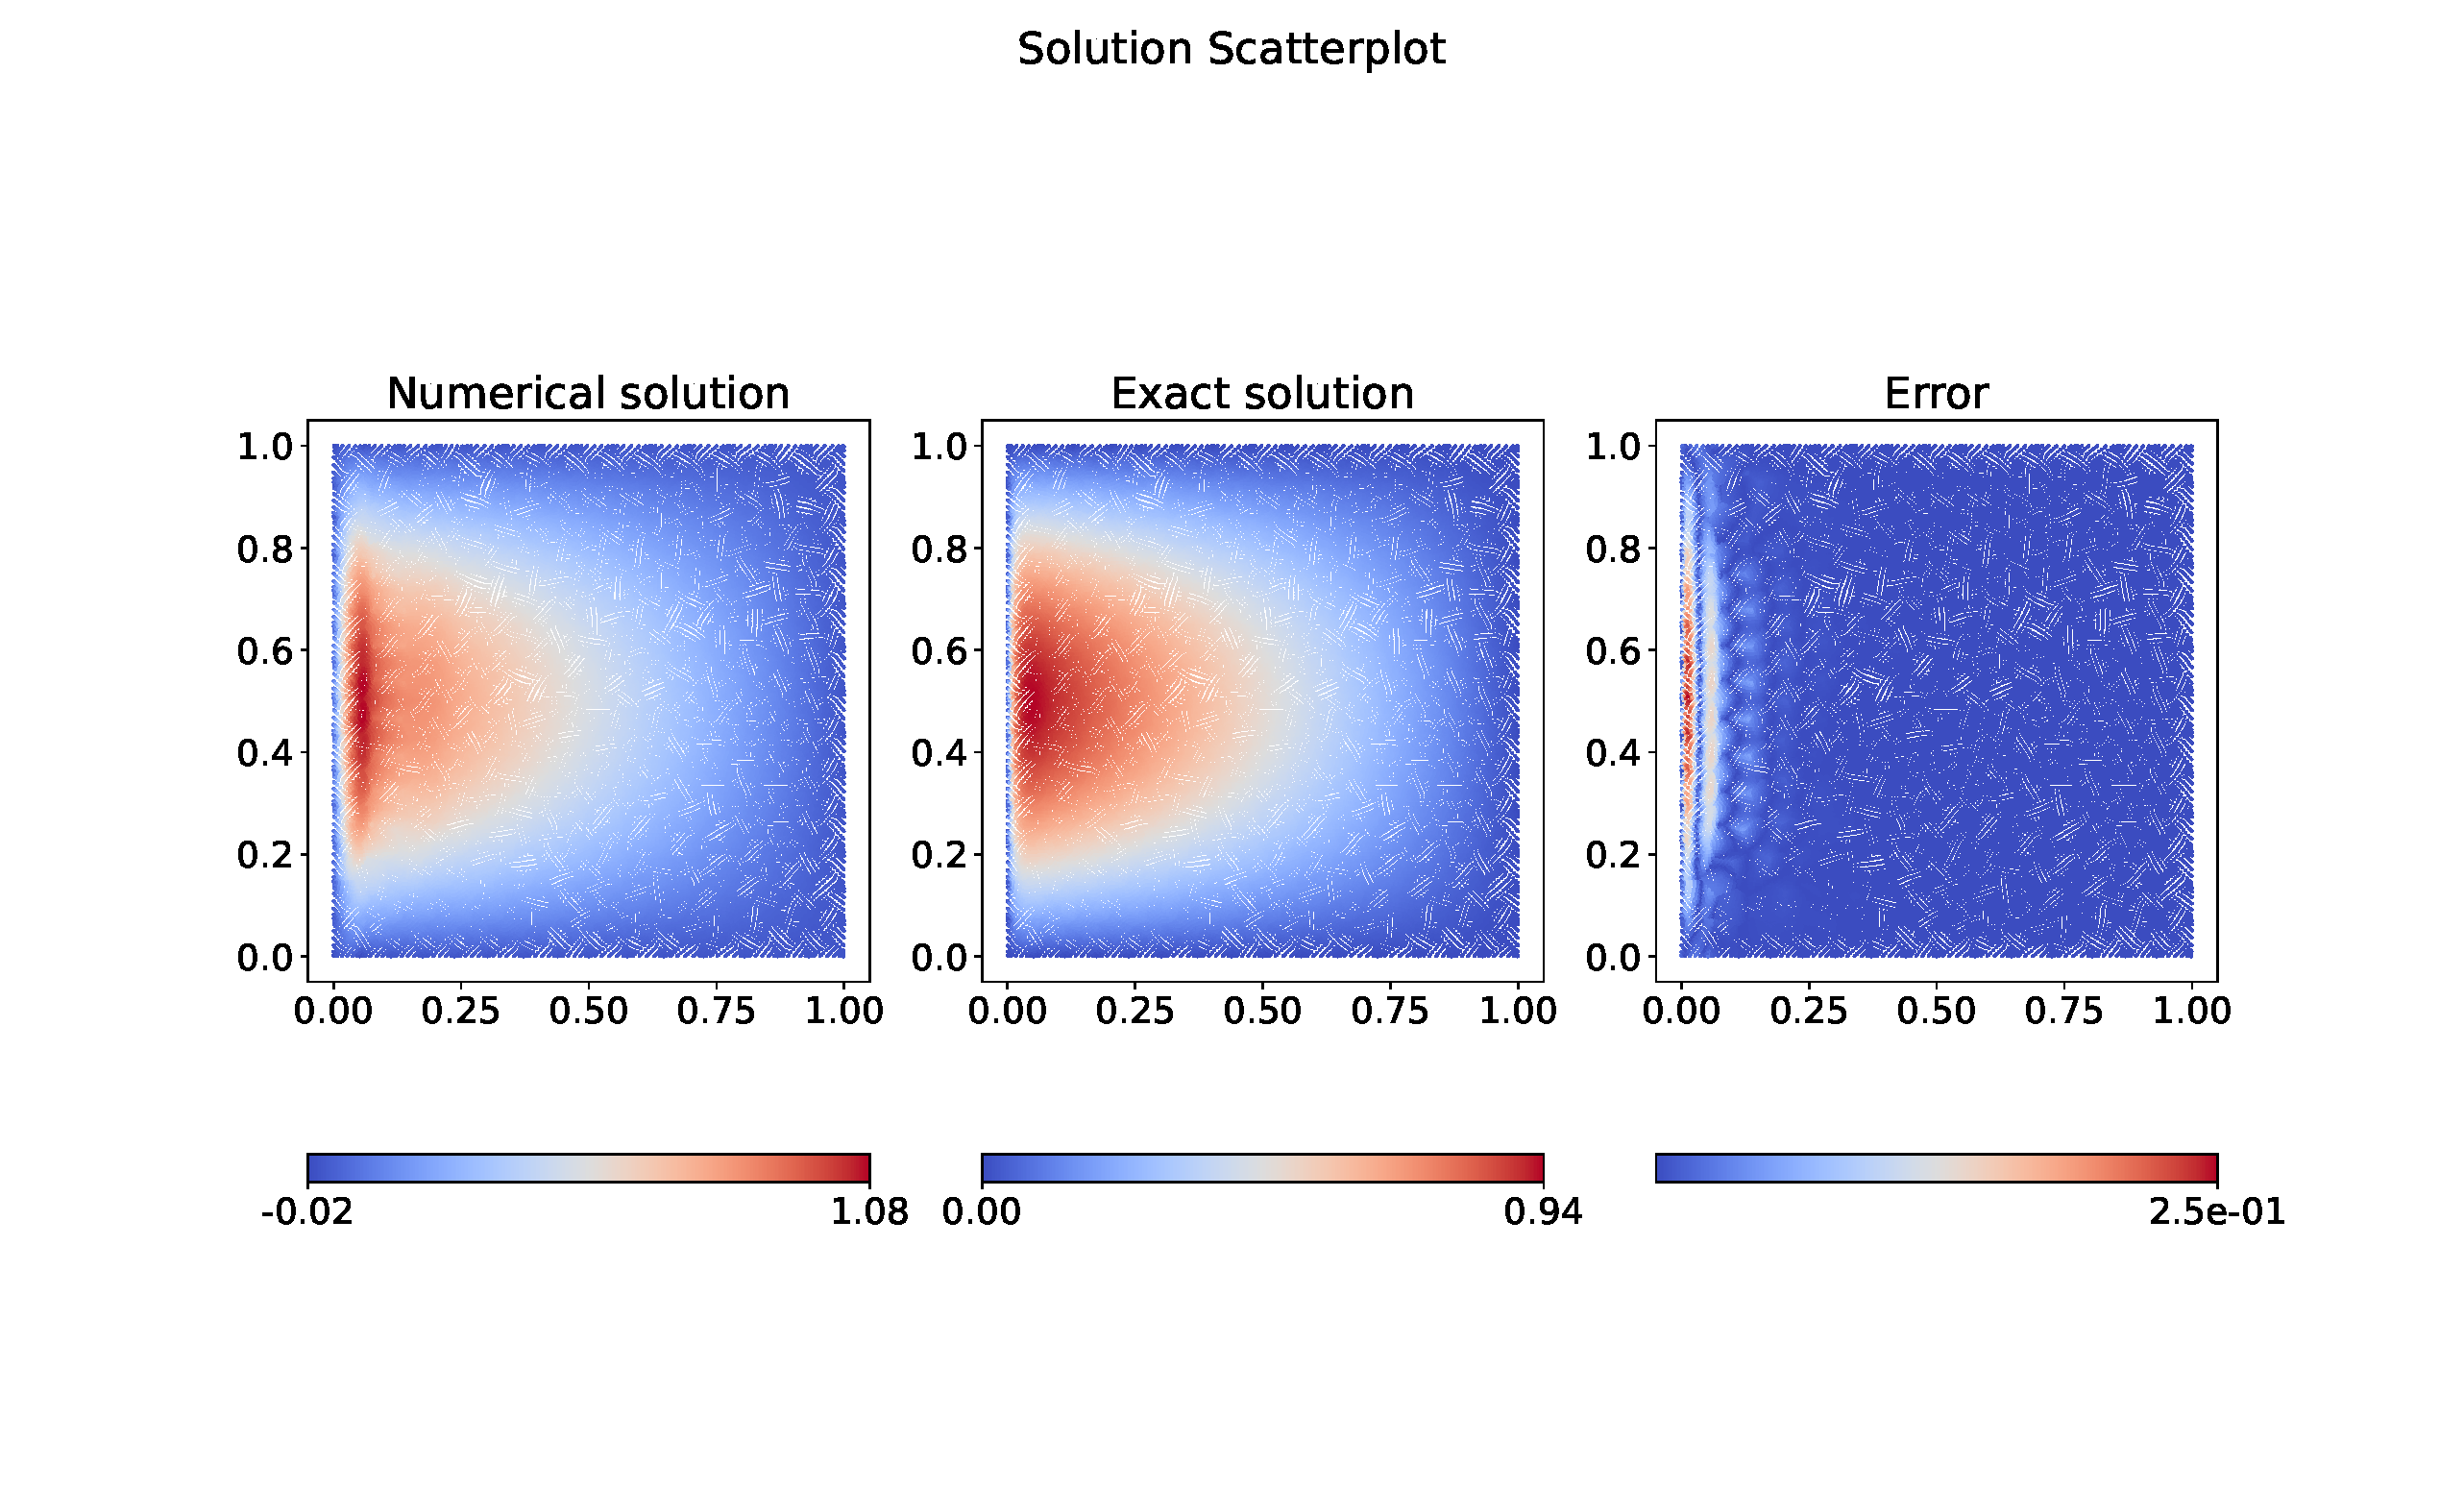
\includegraphics[trim=0cm 2.5cm 0cm 5cm, clip, width=16cm]{square_200_pat.pdf}
    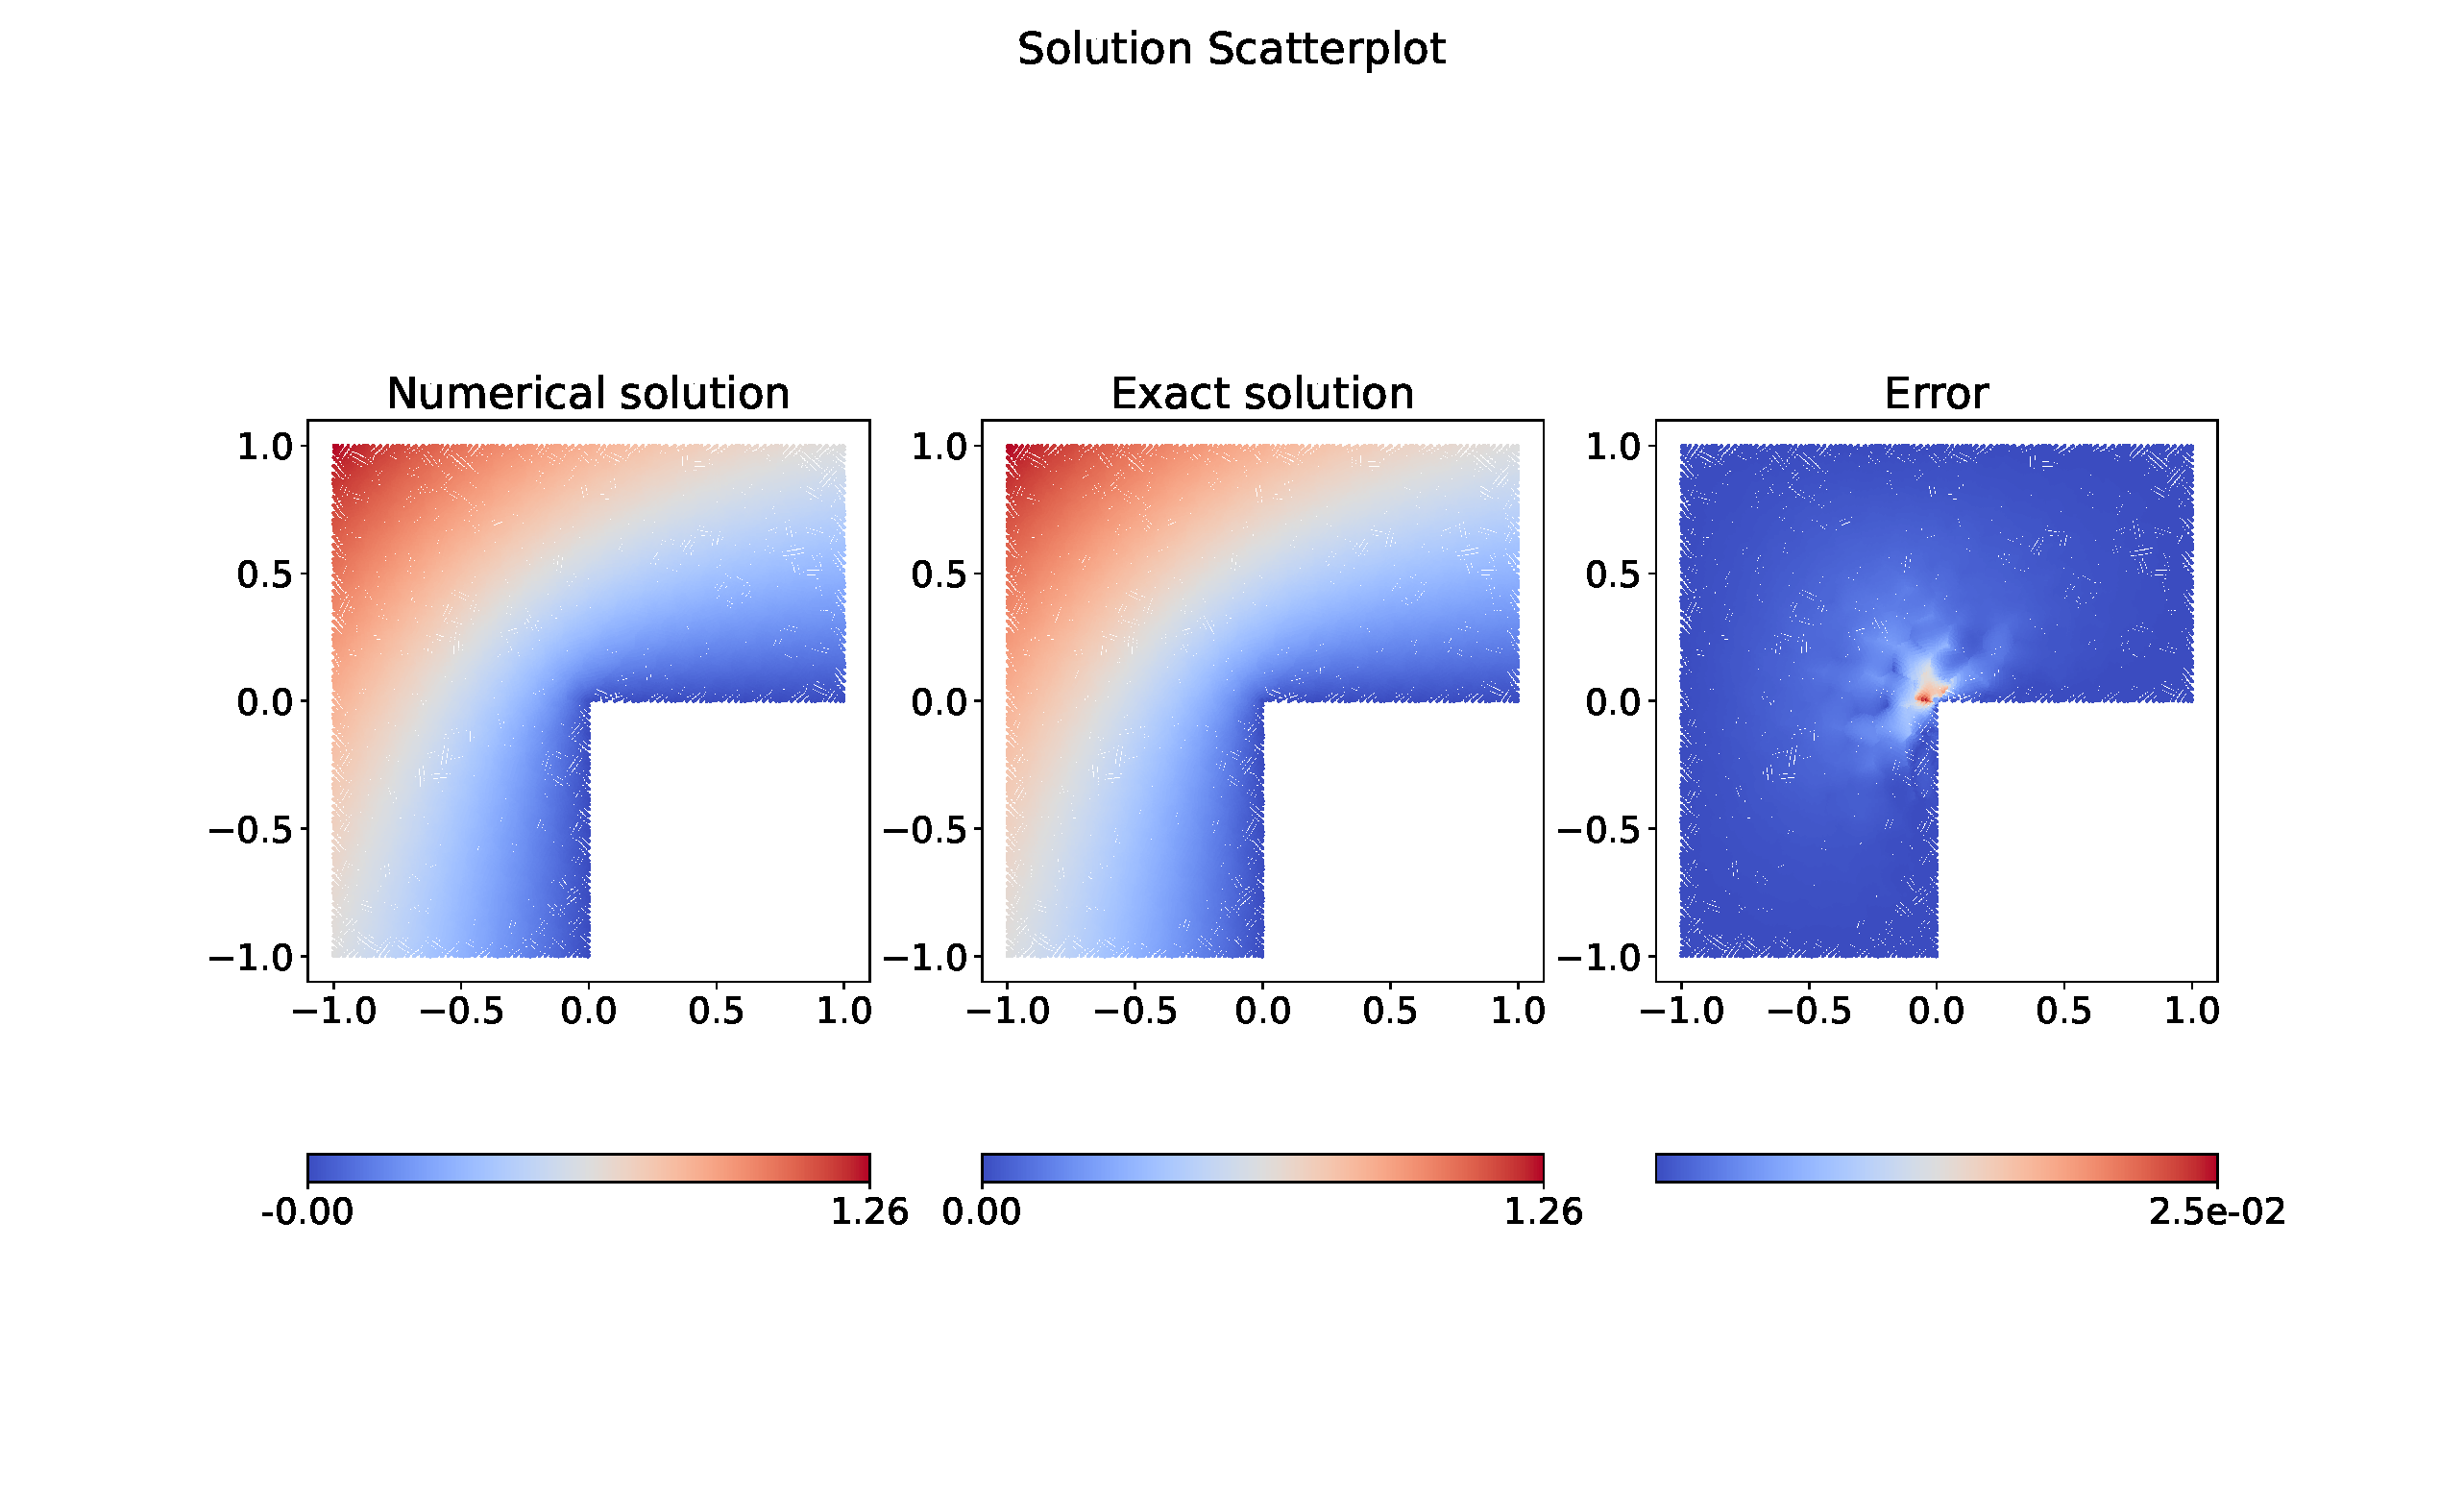
\includegraphics[trim=0cm 2.5cm 0cm 5cm, clip, width=16cm]{lshape_200_pat.pdf}
	\caption{Solution plot over a square domain (top) and an L-shaped domain (bottom), $N = 200$ and $k = 2$.}
\end{figure}